\chapter{Numerical Simulations and Results \label{results}}
In this chapter we discuss the numerical results of the implementation of algorithm \ref{Algorithm} using the PyMongeAmpere library \cite{Merigot2017a} for solving the optimal transport problem. The use of this algorithm allows us to produce results with higher resolutions than previously realised. Plotting the Laguerre diagrams confirms the formation of a front as compared to similar results produced by \cite{Nakamura1994,Cullen1993}. Finally, the validity of the numerical implementation is investigated and performance analysed to assert the suitability of the numerical implementation in providing a solution to equations \ref{EadyModel}.
\section{Physical interpretation of Results \label{laguerre plots}}
Using the plotting process described in section \ref{plotting}. The Laguerre diagrams below show snapshots of frontogenesis and the subsequent evolution of the front. The model was initialised with a grid of $80 \times 40$ points taken from an optimised sampling (see appendix for details) \comments{optimised sampling in appendix} of points in the physical domain $\Gamma = [-L,L]\times[0,H]$ and transformed to geostrophic co-ordinates as explained in \ref{Initpoints}. A summary of parameter values in given in the table below.  For the following results Heun's method described in section \ref{Heun} was used for time-stepping for a time period of 25 days from a randomly generated mesh.
\\
\linebreak
\begin{tabular}{|c|c|c|c|}
	\hline 
	Parameter & Value & Parameter & Value \\
	\hline 
	$L$ & $1 \times 10^6 \ m$ & $H$ & $1 \times 10^4 \ m$ \\ 
	\hline 
	$g$ & $10 \ ms^{-2}$ &	$f$ & $10^{-4} \ s^{-1}$ \\ 
	\hline 
	$N^2$ & $2.5 \times10^{-5} \ s^{-2}$&$\theta_0$ & $300 \ K$ \\ 
	\hline 
	C & $3 \times 10^{-6} \ m^{-1}K$ & $B$ & $0.25$ \\ 
	\hline 
	\end{tabular}
\comments{units for B} 

\begin{figure}[ht!]
	\centering
	\subfloat[]{{\includegraphics[width=0.5\linewidth]{evaluation/laguerre_diagram_thetap_0}}}
	\subfloat[]{{\includegraphics[width=0.5\linewidth]{evaluation/laguerre_diagram_thetap_5}}}\\
	\subfloat[]{{\includegraphics[width=0.5\linewidth]{evaluation/laguerre_diagram_thetap_12}}}
	\subfloat[]{{\includegraphics[width=0.5\linewidth]{evaluation/laguerre_diagram_thetap_18}}}\\
	\caption{Plots of Laguerre Diagrams shaded according to the value of $\theta '$ using a random mesh of $80 \times 40$ points initialised in geostrophic space using \ref{Initpoints} at (a) $0$ days, (b) $2.5$ days (c) $6$ days and (d) $9$ days, $\Gamma = [-L,L]\times[0,H]$, where $L = 1\times10^6$ and $H = 1\times10^4$}
	\label{fig: thetap ldiag}
\end{figure}

\comments{label images with $\theta '$}
In these diagrams we see the growth of the normal mode instability \comments{need to mention before - at $\theta '$ defn?}. Initially (a) the stratification of potential temperature, $\theta '$ is linear, as in the base state. By $2.5$ (b) days we see the instability appear in the form of a wave and by $6$ days a strong front has formed as a large gradient in $\theta '$. We see that warmer air in the upper atmosphere has been come down into the lower regions of the atmosphere. By (d) the front has collapsed again as the normal mode instability loses its predominance. An interesting phenomenon observed after this is that the instability grows again and a secondary front is formed. A cycle then forms of an growing instability in one direction forming a front which is then dissipated and a subsequent instability grows in the opposite direction. Some snapshots of this cycle are shown in the images below. \comments{explanation of tilting??}

\begin{figure}[h]
	\centering
	\subfloat[]{{\includegraphics[width=0.3\linewidth]{evaluation/laguerre_diagram_thetap_22}}}
	\subfloat[]{{\includegraphics[width=0.3\linewidth]{evaluation/laguerre_diagram_thetap_25}}}
	\subfloat[]{{\includegraphics[width=0.3\linewidth]{evaluation/laguerre_diagram_thetap_29}}}\\
	\caption{Plots of Laguerre Diagrams shaded according to the value of $\theta '$ using a random mesh of $80 \times 40$ points initialised in geostrophic space using \ref{Initpoints} at (a) $11$ days, (b) $12.5$ days (c) $14.5$ days, $\Gamma = [-L,L]\times[0,H]$, where $L = 1\times10^6$ and $H = 1\times10^4$}
	\label{fig: front_cycle}
\end{figure}

Diagram (a) shows the formation of the secondary front, (b) shows its collapse and (c) shows the formation of a third front with a reversed gradient in $\theta '$. The front formation is not as clear in these images. As suggested by Dr Cotter this could be due to outlying points which contribute to extreme values of $\theta '$. This skews the colour range as seen in figure \ref{fig: front_cycle}

\begin{figure}[h]
	\centering
	\subfloat[]{{\includegraphics[width=0.3\linewidth]{evaluation/Gpoints_22}}}
	\subfloat[]{{\includegraphics[width=0.3\linewidth]{evaluation/Gpoints_25}}}
	\subfloat[]{{\includegraphics[width=0.3\linewidth]{evaluation/Gpoints_29}}}\\
	\caption{Plots of Geostrophic points at (a) $11$ days, (b) $12.5$ days (c) $14.5$ days}
	\label{Gpoints_front}
\end{figure}

Another interesting visualisation of the result is that of using $v_g$ the cross slice velocity as a colour scale. The diagrams below illustrate this for the same data as in figure \ref{fig: thetap ldiag}. The front formation is a lot clearer in this case especially for the cycle of front formation and collapse.\\

\begin{figure}[ht]
	\centering
	\subfloat[]{{\includegraphics[width=0.5\linewidth]{evaluation/laguerre_diagram_vg_0}}}
	\subfloat[]{{\includegraphics[width=0.5\linewidth]{evaluation/laguerre_diagram_vg_5}}}\\
	\subfloat[]{{\includegraphics[width=0.5\linewidth]{evaluation/laguerre_diagram_vg_12}}}
	\subfloat[]{{\includegraphics[width=0.5\linewidth]{evaluation/laguerre_diagram_vg_18}}}\\
	\caption{Plots of Laguerre Diagrams shaded according to the value of $vg$ using a random mesh of $80 \times 40$ points initialised in geostrophic space using \ref{Initpoints} at (a) $0$ days, (b) $2.5$ days (c) $6$ days and (d) $9$ days , $\Gamma = [-L,L]\times[0,H]$, where $L = 1\times10^6$ and $H = 1\times10^4$}
	\label{fig: vg ldiag}
\end{figure}
\section{Total Energy as a Measurement of Error}
The aim of this section is to validate the results seen in section \ref{laguerre plots} above. With no known analytical solutions to the Eady model for frontogenesis \ref{EadyModel} that we are studying and with no numerical models achieving the resolution we are able to achieve with SG/DA a challenge arises in how to confirm that the results are suitable solutions for the Semi-geostrophic Eady model. In this case, we turn to the total energy to quantify the error in the implementation. This is justified as we know from \cite{Cullen2006a} that the total energy in equation \ref{EadyModel} is conserved. However, given the form of total energy from \ref{energy} as,
\begin{equation}
	E = f^2 \iint \frac{1}{2}\left(X-x\right)^2 - Z\left(z - H/2\right)\textrm{d}x\textrm{d}z
\end{equation}
There is a clear dependence on the values of the points in geostrophic space and the values of the centroids of their corresponding Laguerre cells. This indicates a dependence of the total energy of the system on the numerical solution given by SG/DA at each time-step. The graphs below show the total energy given by a system initialised from a grid of $80 \times 40$ points in geostrophic space (again from applying the transformation to points in physical space by \ref{Initpoints}). This time a regular mesh was used to ensure that the initial energy ($E_0$) was the same for each simulation. \\
\linebreak
The effect of decreasing the time step value was investigated for  both the Forward Euler and Heun time stepping schemes. In the following plots the energy error, $e_t$ is defined as $e_t = E_{t} - E_0$. The final energy error $e_f$ is used to create log-log plots confirming the relationship between the time step used and the numerical error of the implementation. What is most interesting in this is the gradient of the line of best fit, this gives an indication of the order of accuracy of the method. What we expect to see is a gradient, $m$, close to $m=1$ for the Euler method as this is well known to have a linear rate of converge \cite{Griffiths2010} and $m=2$ for the Heun method as this has a quadratic rate of convergence \cite{Griffiths2010}.\pagebreak
\begin{figure}[ht]
	\centering
	\subfloat[]{{\includegraphics[width=0.9\linewidth]{evaluation/energy_5D_euler}}}\caption[Energy Error from implementation of SG/DA via Forward Euler timestepping method for 5 days]{Energy error following the implementation of SG/DA with a Forward Euler time stepping method for 5 days on a regular mesh of $80 \times 40$ points. $\log(\Delta t)$ vs. $\log(e_f)$. The line of best fit has gradient $m = 0.933$, 3.s.f} \label{fig:energy5deuler}
	\subfloat[]{{\includegraphics[width=0.9\linewidth]{evaluation/energy_5D_heun}}}\caption[Energy Error from implementation of SG/DA via Heun timestepping method for 5 days]{ Energy error following the implementation of SG/DA with a Heun time stepping method for 5 days on a regular mesh of $80 \times 40$ points. $\log(\Delta t)$ vs. $\log(e_f)$. The line of best fit has gradient $m = 2.17$, 3.s.f}
	\label{fig:energy5dheun}
\end{figure}
Figures \ref{fig:energy5deuler} and \ref{fig:energy5dheun} indicate promising initial findings. The straight lines in the log-log plots are clear evidence of a power law governing the error - time step relation. Moreover, the gradient values are reasonably close to what we were expecting.\\
\linebreak
The difference in computed values for the gradient to expected values is attributable to the error in applying the Damped Newton Algorithm in DA. To expand, rates of convergence are computed assuming $f(t,\bm{x})$ in $\frac{\textrm{d}\bm{x}}{\textrm{d}t} = f(t,\bm{x})$ has a Taylor expansion \cite{Griffiths2010}. In the case of SG/DA the right hand side includes the implementation of DA which carries error associated with the Damped Newton Algorithm. This is particularly visible in the Heun implementation where the error is significantly smaller. In this case the error associated with DA dominates that associated with the Heun's method and is seen as noise in the energy error curve.\\
\linebreak
Physically we can see that the energy error begins to grow the most between days $4$ and $5$, which coincides with the point where the front seen in figures \comments{frontogensis fig ref} begins to grow most rapidly. To investigate this further the energy error is found for a period of up to $10$ days.
\begin{figure}[ht]
	\centering
	\includegraphics[width=0.9\linewidth]{evaluation/energy_10D_euler}
	\caption[Energy Error from implementation of SG/DA via Forward Euler timestepping method for 10 days]{(a) Energy error following the implementation of SG/DA with a Forward Euler time stepping method for 10 days on a regular mesh of $80 \times 40$ points.\\ (b) $\log(\Delta t)$ vs. $\log(e_f)$. The line of best fit has gradient $m = 0.935$, 3.s.f}
	\label{fig:energy10deuler}
\end{figure}
\begin{figure}[h]
	\includegraphics[width=0.9\linewidth]{evaluation/energy_10D_heun}
	\caption[Energy Error from implementation of SG/DA via Heun timestepping method for 10 days]{(a) Energy error following the implementation of SG/DA with a Heun time stepping method for 10 days on a regular mesh of $80 \times 40$ points.\\ 
		(b) $\log(\Delta t)$ vs. $\log(e_f)$. The line of best fit has gradient $m = 1.88$, 3.s.f}
	\label{fig:energy10dheun}
\end{figure}  
\pagebreak
\section{A Comparison of Time Stepping Methods}
To validate the behaviour exhibited in section \ref{laguerre plots} we look at the behaviour of the Kinetic Energy, Potential Energy and Total Energy with time. We restate the energy in the form \ref{energy},
\begin{equation}
	E= f^2 \iint \frac{1}{2}\left(X-x\right)^2 - Z\left(z - H/2\right)\textrm{d}x\textrm{d}z
\end{equation}
The kinetic energy over the domain $\Gamma$ is defined by,
\begin{equation}
	E_{kin} = \int_\Gamma \ \frac{f^2}{2}(X-x)^2 \ dxdz
\label{KE}
\end{equation}
And the potential energy given by,
\begin{equation}
E_{pot} = \int_\Gamma \ - Z\left(z - H/2\right) \ dxdz
\label{PE}
\end{equation}
We now investigate the evolution of these quantities for a period of 25 days for each time stepping method, initialised with a regular mesh of $80 \times 40$ points transformed to geostrophic co-ordinates as in \ref{Initpoints}.
\begin{figure}[h]
	\centering
	\includegraphics[width=1.0\linewidth]{evaluation/Energy_evolution_euler}
	\caption[Energy evolution for SG/DA with Euler time step scheme]{Energy evolution for SG/DA with Euler time step scheme for regular grid of initialised points}
	\label{fig:energyevolutioneuler}
\end{figure}
Here the cycle of frontogenesis and collapse is much clearer seen in the periodic nature of the Kinetic energy. The graph also shows that energy dissipation in the Forward Euler method is strongest after front formation.
\begin{figure}[h]
	\centering
	\includegraphics[width=1.0\linewidth]{evaluation/Energy_evolution_heun}
	\caption[Energy evolution for SG/DA with Heun time step scheme]{Energy evolution for SG/DA with Heun time step scheme for an initially regular grid of points}
	\label{fig:energyevolutionheun}
\end{figure}
From figure \ref{fig:energyevolutionheun} we see that Heun's method gives numerical results that appear to maintain energy conservation. Comparing the kinetic energy to that of the Forward Euler method there is significantly less damping in the cycle of front formation. The differences in behaviour of kinetic energy is explored further in \ref{fig:energyeulerheuncomparison}.
\begin{figure}[h]
	\centering
	\includegraphics[width=1.0\linewidth]{evaluation/energy_euler_heun_comparison}
	\caption[Comparison of Energy Evolution for SG/DA with Heun/Forward Euler Time Stepping Schemes]{Comparison of energy evolution of solution of SG/EM with SG/DA for Heun and Forward Euler time-stepping schemes over a period of 25 days with a regular grid of initial points}
	\label{fig:energyeulerheuncomparison}
\end{figure}
The comparison shows a significant damping in the amplitude of oscillations in the Forward Euler time stepping scheme compared to the Heun scheme, where the second oscillation appears slightly damped but the third very similar in amplitude to the second. What is also striking is the difference in the periods of oscillation. From \cite{Cullen2006a} we know that the natural period of oscillation show be \comments{period of oscillation} However in their simulations both \cite{Cullen1993,Nakamura1994} achieved periodicities much greater than this\comments{image?}. In \ref{fig:energyeulerheuncomparison} the periodicity is larger, however we see some improvement in Heun's method.
\comments{\cite{Cullen2006a}period of oscillation}
\section{Computational Performance}
\chapter{Unsorted}
\section{Linear Stability Analysis}
Starting from the Eady Model \ref{EadyModel} restated below
\begin{equation}
\begin{aligned}
-fv_g + \frac{\partial \varphi}{\partial x} = 0,\\
\frac{Dv_g}{Dt} + fu -\frac{Cg}{\theta _0}\left(z-H/2\right) = 0,\\
\frac{D\theta'}{Dt} - Cv_g = 0,\\
\frac{\partial \varphi}{\partial z} - g\frac{\theta'}{\theta_0} = 0,\\
\nabla \cdot \bm{u} = 0.
\end{aligned}
\label{EadyModel2}
\end{equation} 
Linearise about a base state given by Hoskins \cite{Hoskins1975},
\begin{equation}
\begin{aligned}
\bar{\theta} &= \theta_0 \frac{N_0^2\theta_0 z}{g} - Cy \\
\bar{\varphi} &= \theta_0 + \frac{N_0^2 z^2}{2}\\
\bar{v}_g &= 0\\
\bar{U} &= \frac{Cg}{f\theta_0}\left(z - H/2\right)\\
\bar{W} &= 0 
\end{aligned}
\end{equation}
Introduce a perturbation and linearise about base state,\\
$u = \bar{U} + u'$, $w = w'$, $v_g =  v_g'$, $\varphi = \bar{\varphi} + \varphi'$, $\theta ' = \bar{\theta} + \theta ''$\\
Introducing the stream function,
\begin{equation}
u' = \frac{\partial \psi}{\partial z},\qquad w' = -\frac{\partial \psi}{\partial x} 
\end{equation}
Looking for normal modes solutions of the form,
\begin{equation*}
q' = \hat{q}(z)\exp^{i \left(kx - \omega t\right)}
\end{equation*}
Equations \ref{EadyModel2} become,
\begin{align}
-f\hat{v}_g + ik\hat{\varphi} = 0,\label{stab1}\\
-i\omega \hat{v}_g + ik\bar{U}\hat{v}_g + f\frac{\text{d}\hat{\psi}}{\text{d}z} = 0,\label{stab2}\\
-i \omega \hat{\theta} + i k \bar{U} \hat{\theta} - ik\frac{N_0^2\theta_0}{g} \hat{\psi} - C\hat{v}_g = 0,\label{stab3}\\
\frac{\text{d}\hat{\varphi}}{\text{d}z} - g\frac{\hat{\theta}}{\theta_0} = 0 \label{stab4},
\end{align}
First eliminating, $\varphi$, equations \ref{stab1} and \ref{stab4} give,
\begin{equation*}
-f\frac{\text{d}\hat{v}_g}{\text{d}z}+ik\frac{\text{d}\hat{\varphi}}{\text{d}z} = 0, \qquad \frac{\text{d}\hat{\varphi}}{\text{d}z} - g\frac{\hat{\theta}}{\theta_0} = 0
\end{equation*}
so that,
\begin{equation}
\hat{\theta} = \frac{f\theta_0}{ikg} \frac{\text{d}\hat{v}_g}{\text{d}z}
\label{thetahat}
\end{equation}
Rearranging equation \ref{stab3}
\begin{equation}
i\left( k \bar{U} - \omega \right) \hat{\theta} - ik\frac{N_0^2\theta_0}{g} \hat{\psi} - C\hat{v}_g = 0
\label{stab3.1}
\end{equation}
Eliminating $\hat{\theta}$ using \ref{thetahat}
\begin{equation*}
\frac{f\theta_0}{kg}\left( k \bar{U} - \omega \right)  \frac{\text{d}\hat{v}_g}{\text{d}z} - ik\frac{N_0^2\theta_0}{g} \hat{\psi} - C\hat{v}_g = 0
\end{equation*}
from equation \ref{stab2} we have
\begin{equation}
i\left( k \bar{U} - \omega \right) \hat{v}_g - f \frac{\text{d}\hat{\psi}}{\text{d}z} = 0
\label{stab2.1}
\end{equation}
differentiating this expression we find
\begin{equation*}
ik \frac{\text{d}\bar{U}}{\text{d}z} \hat{v}_g + i(k\bar{U}-\omega)\frac{\text{d}\hat{v}_g}{\text{d}z} + f\frac{\text{d}^2{\psi}}{\text{d}z^2} = 0 
\end{equation*}
Substituting this expression with \ref{stab2.1} into \ref{stab3.1}, noting that,
\begin{equation*}
(k\bar{U}-\omega)\frac{\text{d}\hat{v}_g}{\text{d}z} = if\frac{\text{d}^2{\psi}}{\text{d}z^2} + \frac{fk}{i(k\bar{U}-\omega)}\frac{\text{d}\bar{U}}{\text{d}z}\frac{\text{d}\hat{\psi}}{\text{d}z}
\end{equation*}
\begin{equation*}
\frac{f\theta_0}{kg}\left(if\frac{\text{d}^2{\psi}}{\text{d}z^2} + \frac{fk}{i(k\bar{U}-\omega)}\frac{\text{d}\bar{U}}{\text{d}z}\frac{\text{d}\hat{\psi}}{\text{d}z}\right) - \frac{ik N_0^2\theta_0\hat{\psi}}{g} + \frac{Cf}{i(k\bar{U}-\omega)}\frac{\text{d}\psi}{\text{d}z} =0
\end{equation*}
Rearranging gives,
\begin{equation*}
-\frac{f^2\theta_0}{kg}(k\bar{U}-\omega)\frac{\text{d}^2{\psi}}{\text{d}z^2}+\left(Cf+\frac{f^2\theta_0}{g}\frac{\text{d}\bar{U}}{\text{d}z}\right)\frac{\text{d}\hat{\psi}}{\text{d}z}+\frac{k N_0^2\theta_0}{g}(k\bar{U}-\omega)\hat{\psi}=0
\end{equation*}
\begin{equation*}
-f^2\theta_0(k\bar{U}-\omega)\frac{\text{d}^2{\psi}}{\text{d}z^2}+2Cfkg\frac{\text{d}\hat{\psi}}{\text{d}z}+k^2 N_0^2\theta_0(k\bar{U}-\omega)\hat{\psi}=0
\end{equation*}
We reformulate this as a matrix eigenvalue problem for $\omega$
\begin{equation}
-f^2\theta_0\bar{U}\frac{\text{d}^2{\psi}}{\text{d}z^2}+2Cfkg\frac{\text{d}\hat{\psi}}{\text{d}z}+k^2 N_0^2\theta_0\bar{U}\hat{\psi}=\omega \left(k^2N_0^2\theta_0\hat{\psi}-f^2\theta_0 \frac{\text{d}^2{\psi}}{\text{d}z^2}\right)
\label{stabanalysis}
\end{equation}
Introducing a second order finite difference scheme for $\psi$
\begin{equation*}
\begin{aligned}
\frac{\text{d}^2{\hat{\psi}}}{\text{d}z^2} = \frac{\psi_{i-1} - 2\psi_i + \psi_{i+1}}{h^2}\\
\frac{\text{d}\hat{\psi}}{\text{d}z} = \frac{\psi_{i-1} - \psi_{i+1}}{2h}
\end{aligned}
\end{equation*}
Equation \ref{stabanalysis} becomes
\begin{equation}
\begin{aligned}
-f^2\theta_0\bar{U}_i\left(\frac{\psi_{i-1} - 2\psi_i + \psi_{i+1}}{h^2}\right)+2Cfkg\left(\frac{\psi_{i-1} -f \psi_{i+1}}{2h}\right)+k^3 N_0^2\theta_0\bar{U}_i\psi_i= \\
\omega\left(k^2N_0^2\theta_0\psi_i-f^2\theta_0\left(\frac{\psi_{i-1} - 2\psi_i + \psi_{i+1}}{h^2}\right)\right)
\end{aligned}
\end{equation}
Discretising the interval $[0,H]$ into $N$ points with step size $h$ we can recast this as an eigenvalue problem,
\begin{equation*}
A\bm{\psi} = \omega B\bm{\psi}
\end{equation*}
to find eigenvalues $\omega$ with corresponding eigenvectors $\bm{\psi} = \left(\psi_1, ... , \psi_{N-2}\right)$. Since the boundary condition gives $\psi = 0$ on $z = 0, H$, $\psi_0 = \psi_N = 0$ so these are omitted from the $\hat{\phi}$ vector but considered in the finite difference schemes for $\psi_1$ and $\psi_{N-1}$
The coefficients matrix $A$ are given by
\begin{equation}
\begin{aligned}
\psi_{i-1}:& \quad -\frac{-f^2\theta_0k\bar{U}_i}{h^2} - \frac{Cfkg}{h}\\
\psi_i:& \quad \frac{2f^2\theta_0k\bar{U}_i}{h^2} + k^3N_0^2\theta_0\bar{U}_i\\
\psi_{i+1}:& \quad \frac{-f^2\theta_0k\bar{U}_i}{h^2} + \frac{Cfkg}{h}\\
\end{aligned}
\end{equation}
$i: 1 \rightarrow N-2$ with $\psi_0 = \psi_{N}$. The coefficients of matrix $B$ are given by,
\begin{equation*}
\begin{aligned}
\psi_{i-1}:& \quad -\frac{f^2\theta_0}{h^2}\\
\psi_i:& \quad k^2N_0^2\theta_0 + \frac{2f^2\theta_0}{h^2}\\
\psi_{i+1}:& \quad -\frac{f^2\theta_0}{h^2}\\
\end{aligned}
\end{equation*}
\begin{figure}[h]
	\centering
	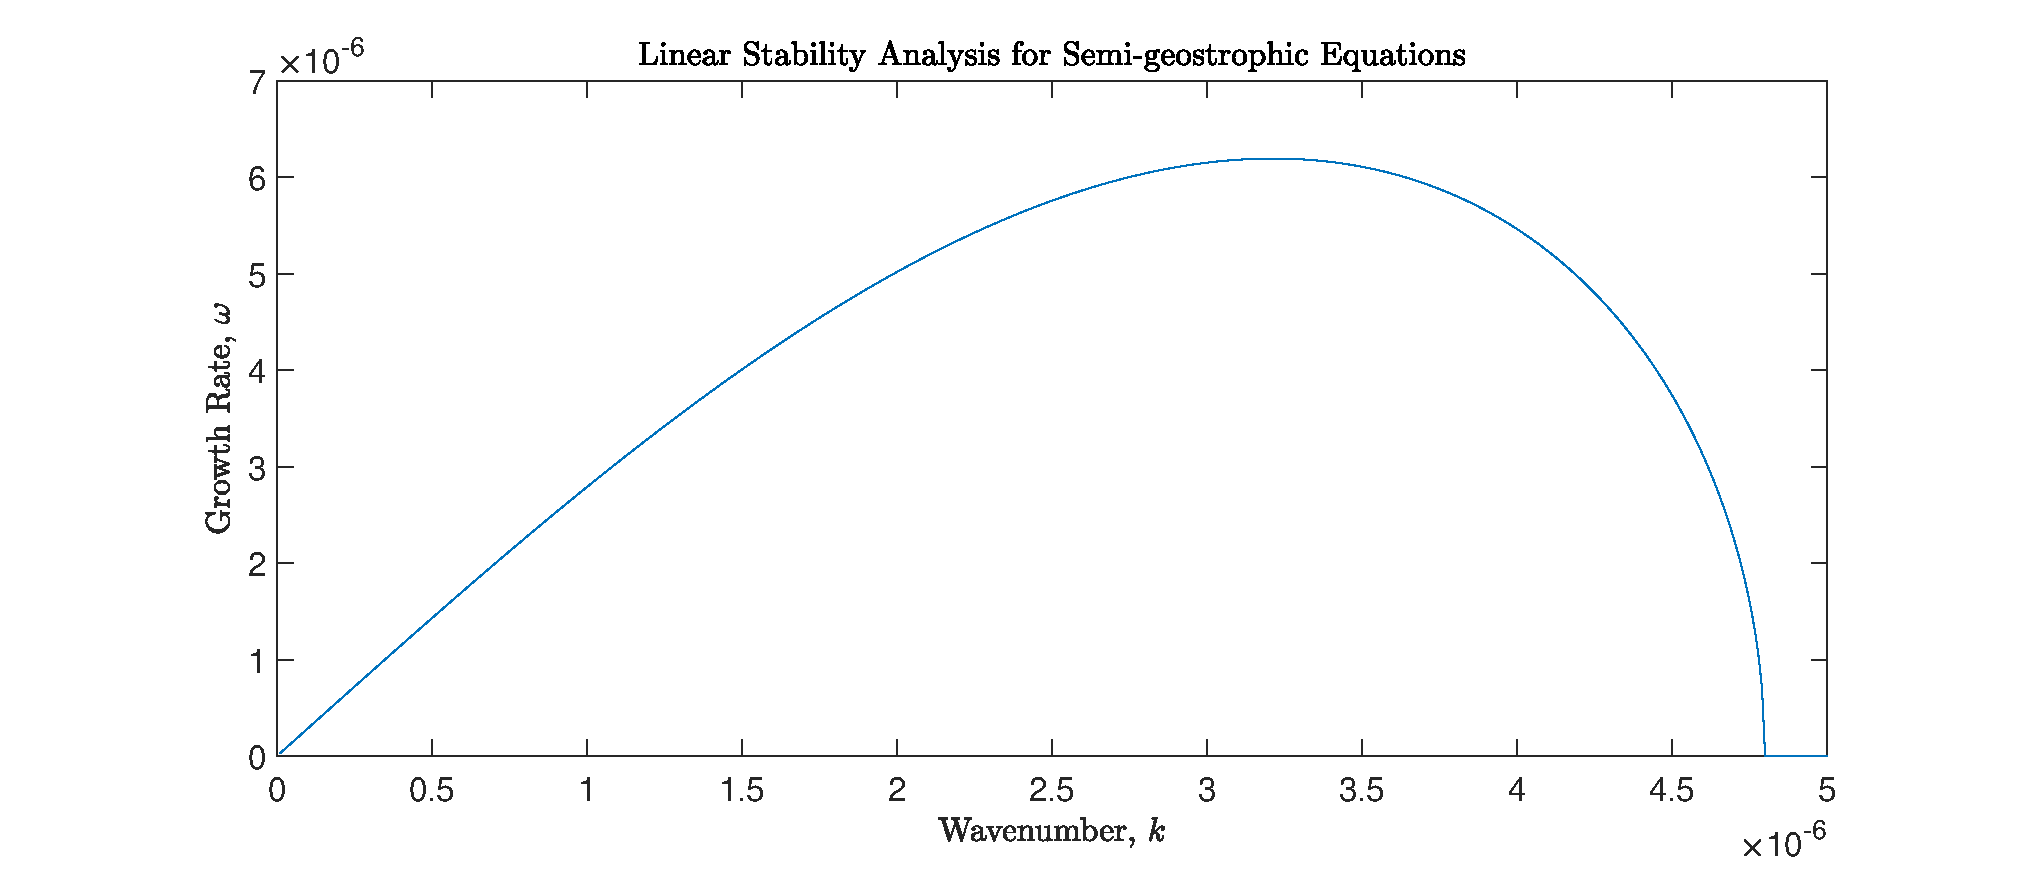
\includegraphics[width=\linewidth]{project/Linear_stability_analysis}
	\caption[Linear stability analysis results for the semi-geostrophic equations]{Plot showing growth rate, $\omega$ against wavenumber $k$ for the Eady model of the semi-geostrophic equations}
	\label{fig:linearstabilityanalysis}
\end{figure}
\section{Calculation of Moments}
For the implementation of the numerical algorithm for frontogenesis and subsequent analysis of its suitability, the moments of \comments{word choice} the cells are required. Consider a point in geostrophic space $\bm{Y} = \left(X,Z\right)$ in the fundamental domain and corresponding weight $\psi$ for which the Laguerre cell is $A = \mathrm{Lag}_{\bm{Y}}(\psi)$
\begin{description}
	\item [$\bm{O^{th}}$ Moment] 
	\begin{equation}
		M_0 = \int_A dxdz
	\end{equation}
	\item[$\bm{1^{st}}$ Moment]
	\begin{equation}
	M_{1x} = \int_A x dxdz, \qquad M_{1z} = \int_A z dxdz
	\end{equation}
	\item[$\bm{2^{nd}}$ Moment]
	\begin{equation}
	M_{2x} = \int_A x^2 dxdz, \qquad M_{2z} = \int_A z^2 dxdz, \qquad M_{2xz} = \int_A xz dxdz
	\end{equation}	
\end{description}

\subsection{Considerations for Periodic Boundary Conditions}
In implementing the moment calculations the periodicity of the domain needs to be carefully considered. For example, consider a point in geostrophic space $\left(X, Z\right)$ in the fundamental domain and corresponding weight $\psi$ it is possible that if $X$ lies close to one of the limit points of the interval $[-L,L]$, that the centroid of the Laguerre cell associated with this point is exterior to the fundamental domain.
\section{Ideas for extension}
